\chapter{Markov Chains}

\section{Introduction to Markov Chains}
	
	\subsection{Stochastic Processes}

	Before we consider the concept of Markov Chains, we will introduce the notion of a \emph{stochastic 
	process}. 
	\begin{definition}[Stochastic Process]
		A \emph{stochastic process} $X \equiv (X_t)_{t \in T}$ with \emph{index set} $T$ is a collection 
		of random variables indexed by the elements of $T$, where $\forall t \in T. \mathrm{range}(X_t) 
		= \mathcal{I}$ is the so-called \emph{state space}. 
	\end{definition}
	\begin{comment}
		The random variables of a stochastic process do not necessarily conform entirely with the 
		definition given in Chapter 1. The state space $\mathcal{I}$ can have $\mathcal{I} \not\subseteq
		\mathbb{R}$, which is what violates the earlier definition; for example, they can take values from
		higher powers of the real numbers.
	\end{comment}
	The \emph{index set} $T$ is often a subset of the real numbers, which has had the effect that stochastic 
	processes are commonly thought of as being indexed by `time', i.e.\ that they model the development of
	a random variable over time, which is also why we speak of the difference $X_t - X_{t'}$ as the 
	`increment' between $t, t'$. This notion is more proper for the special case of stochastic processes known
	as Markov Chains.

	\subsection{Markov Chains}
	
	Before we define Markov Chains, we first need to clarify the notion of a probability distribution over an
	enumerable\footnote{i.e\ finite or countably infinite} set $\mathcal{I}$:
	\begin{definition}[Probability Distribution]
		A function $\mu \in \mathcal{I} \rightarrow \mathbb{R}$ is a \emph{probability distribution},
		or a \emph{probability vector} if 
		\begin{itemize}
			\item $\forall i \in \mathcal{I}. \mu_i \coloneqq \mu(i) \in [0,1]$.
			\item $\sum_{i \in \mathcal{I}} = 1$.
		\end{itemize}
		For the purposes of this course, these probability vectors will always be \emph{row} vectors.
	\end{definition}

	\begin{definition}[Markov Chain]
		A \emph{Markov Chain} on state space $\mathcal{I}$, with initial probability distribution 
		$\mu$, and transition matrix $\mathbf{P}$ is a stochastic process with state space $\mathcal{I}$ 
		and index set $\mathbb{N}_0$ with the following additional axioms:
		\begin{itemize}
			\item $\mathcal{I}$ is \emph{enumerable}.
			\item $\forall i \in \mathcal{I}. \mathbb{P}(X_0 = i) = \mu_i$.
			\item The following, known as the \emph{Markov Property}, holds:
			$$
				\forall i  \in \mathcal{I}, t \in \mathbb{N}_0. 
				\mathbb{P}(X_{t+1} = i | X_{0}= i_0 \hdots X_{t} = i_t) = 
				\mathbb{P}(X_{t+1} = i | X_t = i_t) \coloneqq P_{i_t, i} \text{ is constant.}
			$$
		\end{itemize}
	\end{definition}
	The Markov Property ensures that any one random variable $X_{t}$ is only dependent on its `prædecessor',
	that is, the variable $X_{t-1}$. One can model a different number of preceding dependencies 
	by re-modelling the state space as $\mathcal{I}^k$ , and have each such new state represent the latest 
	$k$ states the Markov Chain went through, or by having a higher-order tensor with transition
	probabilities.
	
	\subsubsection{Further Notational Details}
		If the state space $\mathcal{I}$ is finite, that is, if there is an enumeration $e: \mathcal{I} 
		\rightarrow \{1\hdots n\}$ for some $n$, we will in particular represent a Markov chain in two 
		ways, firstly by explicitly giving its transition matrix 
		$$
			\mathbf{P} = 
			\begin{pmatrix}
				P_{e^{-1}(1),e^{-1}(1)} & \hdots & P_{e^{-1}(1), e^{-1}(n)} \\
				\vdots & \ddots & \vdots \\
				P_{e^{-1}(n),e^{-1}(1)} & \hdots & P_{e^{-1}(n), e^{-1}(n)}
			\end{pmatrix}
		$$
		and secondly by drawing a node-and-link diagram of a directed graph with weighted edges, where
		each vertex is a state $i \in \mathcal{I}$, and each edge $(i, j)$ is weighted by $P_{i,j}$. \par
		For example, we may consider the carbohydrate component of the lunch served in a College's hall
		as modelled by a Markov Chain over state space $\mathcal{I} = \{\mathrm{Pasta}, \mathrm{Potatoes},
		\mathrm{Rice}\}$, where we enumerate the states in alphabetical order. Then the transition matrix 
		of our `College Carbs' Markov chain might be the following:
		$$
			\mathbf{P} = 
			\begin{pmatrix}
				0 & \sfrac{1}{2} & \sfrac{1}{2} \\
				\sfrac{1}{4} & 0 & \sfrac{3}{4} \\
				\sfrac{3}{5} & \sfrac{2}{5} & 0 
			\end{pmatrix}
		$$
		Then the state transition diagram would be visualised as follows: \\
		\begin{center}
		\begin{tikzpicture}
			\draw node[circle,minimum size=2.0cm, draw] at (0cm,0cm) (pasta) {Pasta};
			\draw node[circle,minimum size=2.0cm, draw] at (4cm,0cm) (tater) {Potatoes};
			\draw node[circle,minimum size=2.0cm, draw] at (2cm,4cm)  (rice) {Rice};
			\draw[->] (pasta) edge [bend left] node[pos=0.5, left] {$\sfrac{1}{2}$} (rice);
			\draw[->] (pasta) edge node[pos=0.5, above] {$\sfrac{1}{2}$} (tater);
			\draw[->] (tater) edge [bend left] node[pos=0.5, below] {$\sfrac{1}{4}$} (pasta);
			\draw[->] (tater) edge  node[pos=0.5, left] {$\sfrac{3}{4}$} (rice);
			\draw[->] (rice) edge node[pos=0.5, right] {$\sfrac{3}{5}$} (pasta);
			\draw[->] (rice) edge [bend left] node[pos=0.5, right] {$\sfrac{2}{5}$} (tater);
		\end{tikzpicture}
		\end{center}

		Regardless of the state space's cardinality, we will denote by $p_i(t)$ the probability that
		at time $t$, the Markov Chain will be in state $i \in \mathcal{I}$. This notation invites the
		use of $\mathbf{p}(t)$ as $(p_{i_0}, p_{i_1} \hdots)$ as probability distribution at time $t$, 
		that is, the vector containing at index $k$ the probability that the Markov Chain will be in state
		$i_k$ at time $t$. Note that, with this convention, clearly $\mathbf{p}(0) = \mu$.\par 
		This convention also allows us to calculate $\mathbf{p}(t+1)$ as $\mathbf{p}(t) \cdot \mathbf{P}$, 
		that is $p_i(t+1) = \sum_{j \in \mathcal{I}} p_{j} \cdot P_{j,i}$, by the law of total probability,
		from which (due to the Markov Property) it also follows that $\forall k \in \mathbb{N}_0. 
		\mathbf{p}(t+k) = \mathbf{p}(t) \cdot \mathbf{P}^k$, i.e.\ $\mathbf{P}_{i,j}^k = \mathbb{P}(X_k=j
		| X_0 = i)$.


	\subsection{Stopping and Hitting Times}
		We now consider the concept of \emph{stopping} and {hitting times}, which intuitively model the
		amount of time that passes before a certain event occurs. Before defining these notions, though,
		we will formalise the concept of information available at a given time $t = n$. To this end, we 
		define a \emph{filtration} as follows:
		\begin{definition}[$\sigma$-Algebra]
			Given any set $X$, a $\sigma$\emph{-algebra} $\mathcal{A}$ of $X$ is a subset $\mathcal{A} 
			\subseteq \mathcal{P}(X)$ that satisfies
			\begin{itemize}
				\item $X \in \mathcal{A}$,
				\item $\mathcal{A}$ is closed under complementation and
				\item $\mathcal{A}$ is closed under union.
			\end{itemize}
		\end{definition}
		\begin{comment}
			We say that, if $\mathcal{A}$ and $\mathcal{B}$ are $\sigma$-algebræ over a set $X$,
			if $\mathcal{B} \subseteq \mathcal{A}$, $\mathcal{B}$ is a 
			\emph{sub-}$\sigma$\emph{-algebra} of $\mathcal{A}$.
		\end{comment}
		\begin{definition}[Filtration]
			Let $(\Omega, \mathcal{A}, \mathbb{P})$ be a probability space, and $(\mathcal{I}, 
			\preceq)$ a totally ordered index set. Then note that $\mathcal{A}$ is a 
			$\sigma$-algebra of $\Omega$, then let $\mathbb{F} \coloneqq (\mathcal{F}_i)_{i \in 
			\mathcal{I}}$ be a family of sub-$\sigma$-algebræ of $\mathcal{A}$. We say that 
			$\mathbb{F}$ is a \emph{filtration} iff, for all $i, j \in \mathcal{I}$ such that $i 
			\preceq j$, $\mathcal{F}_i \subseteq \mathcal{F}_j$.
		\end{definition}

		We can now continue to define the notion of a stopping time, which formalises the idea of 
		a random process terminating once a certain event occurs.
		\begin{definition}[Stopping Time]
			A random variable $\tau$ ranging over a discrete $T$ (which is totally ordered by 
			$\leq$) is a \emph{stopping time} for the stochastic process $(X_t)_{t \in T}$ with state 
			space $\mathcal{I}$ iff the filtration $\mathbb{F}$, defined as 
			$(\mathcal{F}^{\cup}_t)_{t \in T}$, where 
			for each $t \in T$, we define $\mathcal{F}^\cup_t$ as the closure under union and 
			complementation of $\mathcal{F}_t$ recursively defined by 
			$\mathcal{F}_{\mathrm{succ} t} \coloneqq \{X_{\mathrm{succ} t} = i : i \in \mathcal{I}\} 
			\cup \mathcal{F}_t$ with $\mathcal{F}_{t_0} = \{\varnothing, T\rightarrow\mathcal{I}\} 
			\cup \{X_{t_0} = i : {i} \in \mathcal{I}\}$, where $t_0 \coloneqq \inf T$, 
			has $\forall t \in T. \langle\tau = t\rangle \in \mathcal{F}^{\cup}_t.$
		\end{definition}
		\begin{comment}
			In layman's terms, this mouthful simply means that the event $\tau = t$ only depends on the
			variables $X_{t'}$ for $t' \leq t$.
		\end{comment}
		Stopping times formalise the idea of stopping a stochastic process in the sense that it only makes 
		sense for a stochastic process to terminate once the desired event has occured for certain, which
		means that at time $t$, only the information from the sub-process $(X_{t'})_{t' \leq t}$ should be
		available. So, for our example of the `College Carbs' Markov Chain, a valid stopping time might be
		$\tau = \inf(t : X_t = \mathrm{Pasta})$, i.e.\ the first time that Pasta was 
		served, but not $\tau'= \inf(t : X_t=\mathrm{Pasta}\land X_{t+1}=\mathrm{Rice})$.
		\par
		Having now defined the notion of stopping times, we can go on to consider hitting times, which 
		measure the expected time before the process reaches a certain state.
		\begin{definition}[Hitting and Return Times]
			For a stochastic process $(X_t)_{t \in T}$ over state space $\mathcal{I}$, we define the 
			\emph{hitting time} $h_{i,j}$ from state $i$ to state $j$ as $h_{i,j} \coloneqq 
			\mathbb{E}_i(\tau_j) = \mathbb{E}(\tau_j | X_{t_0} = i)$, where $\tau_j \coloneqq 
			\inf(t \in T : X_t = j)$. \par
			We further define the \emph{first return time} to state $i$ as $\mathbb{E}_i(\tau_i^+) = 
			\mathbb{E}(\tau_i^+ | X_{t_0} = i)$ where $\tau_i^+ \coloneqq \inf(t > t_0 : X_t = i)$.
			\par
			Note that in both above definitions we have taken $t_0 \coloneqq \inf T$.
		\end{definition}
		
		From these definitions, we should note a few things. Firstly, $\forall i\in \mathcal{I}. h_{i,i}=
		t_0$, while $\mathbb{E}_i(\tau_i^+) > t_0$. Secondly, we have that, if $i \neq j$ are two distinct
		states, then $h_{i,j} = \mathbb{E}_i(\tau_j^+)$. Finally, which follows trivially from the Markov 
		Property,
		\begin{lemma}
			If $X$ is a Markov Chain over state space $\mathcal{I}$, that is, $T = \mathbb{N}_0$, 
			the hitting times of the states in the state space are solutions to the 
			set of linear equations
			$$
				\mathbb{E}_i(\tau_j^+) = 1 +\sum_{k\in\mathcal{I}} \mathbb{E}_k(\tau_j) 
				\cdot P_{i, k}
			$$
		\end{lemma}
		the proof of ithem actually being the minimal non-negative solutions is beyond the scope of these 
		notes. However, we can prove the following result:
		\begin{lemma}
			For a Markov chain $(X_t)_{t \in \mathbb{N}_0}$ with state space $\mathcal{I}$, and 
			$\tau_i \coloneqq \inf(t : X_t = i)$, $\tau_i$ is a stopping time for $(X_t)_{t\in 
			\mathbb{N}_0}$.
		\end{lemma}
		\begin{proof}
			For any $i \in \mathcal{I}$, we have that 
			\begin{align*}
				\langle\tau_i = n\rangle &= \langle \forall 0 \leq t < n . X_t \neq i \land
				X_n=i\rangle \\
				&= \langle X_n = i\rangle \cap \bigcap_{t=0}^{n-1} \langle X_t \neq i \rangle \\
			\end{align*}
			Since the member $\mathcal{F}^\cup_n$ of the filtration $\mathbb{F}$ as defined before is
			closed under complementation and union, it is also closed by intersection. Therefore the 
			event $\langle \tau_i = n \rangle$ is in $\mathcal{F}_n^{\cup}$.
		\end{proof}
		
	\subsection{Properties of Markov Chains}
		
		\subsubsection{Irreducibility and Stationarity}
			\begin{definition}
				We say that a Markov Chain $(X_t)_{t \in \mathbb{N}_0}$ with transition matrix 
				$\mathbf{P}$ and state space $\mathcal{I}$ is \emph{reducible} if $\exists i,j 
				\in \mathcal{I}. \forall n \in \mathbb{N}. (\mathbf{P}^n)_{i,j} = 0$, otherwise 
				it is \emph{irreducible}. 
			\end{definition}
			\begin{comment}
				If for states $i,j$ $\exists n \in \mathbb{N}. (\mathbf{P}^n){i,j} > 0$, we say 
				that state $j$ is accessible from $i$. When $j$ is accessible from $i$ and vice 
				versa, we say that the states $i,j$ \emph{communicate}. Note that sometimes, any 
				state $i$ is taken to be accessible from itself, in which case each instance of 
				$\mathbb{N}$ above should be replaced by $\mathbb{N}_0$. This notion does not 
				make more Markov chains irreducible. To see why, consider a Markov chain that is 
				reducible under the definition given above, but suppose having each state be 
				accessible from itself makes it irreducible. Then, if under the first definition 
				$i, j$ did not communicate, they must be equal, $i = j$. However, this implies 
				that $\forall i \neq j. \exists n,m \in \mathbb{N}. (\mathbf{P}^n)_{i,j} > 0 
				\land (\mathbf{P}^m)_{j,i} > 0$. Therefore, $\forall i. \exists n,m > 0. 
				(\mathbf{P}^{n+m})_{i,i} > 0$, violating the original hypothesis.
			\end{comment}
			For example, if we consider Markov chains over the state space $\mathcal{I} \coloneqq 
			\{i,j,k,l\}$, the first one, given below is \emph{reducible}, as there are two 
			\emph{communicating classes}, that is, there is a partition of the state space 
			$\mathcal{I}$ of cardinality $> 1$ in which, for every set of states, all states 
			communicate, but for every other set of states there is one state that does not 
			communicate with them. Here, $\{k,l\}$ is a \emph{closed} communicating class, that is, 
			no state outside it is accessible from within it. 
			\ \\\ \\ 
			\noindent
			\begin{tabular}{C{0.5\textwidth}C{0.5\textwidth}}
				\begin{tikzpicture}
					\draw node[circle, draw, minimum size=0.75cm] (i) {$i$};
					\draw node[circle, draw, minimum size=0.75cm] 
					[above of=i, node distance=3cm] (j) {$j$};
					\draw node[circle, draw, minimum size=0.75cm] 
					[right of=j, node distance=3cm] (k) {$k$};
					\draw node[circle, draw, minimum size=0.75cm] 
					[right of=i, node distance=3cm] (l) {$l$};
					\draw[->] (i) edge [loop, out=190, in=260, looseness=5] 
					node[left] () {$\sfrac{1}{4}$} (i);
					\draw[->] (j) edge [loop, out=100, in=170, looseness=5] 
					node[left] () {$\sfrac{1}{3}$} (j);
					\draw[->] (k) edge [loop, out=80, in=10, looseness=5] 
					node[right] () {$\sfrac{1}{2}$} (k);
					\draw[->] (l) edge [loop, out=350, in=280, looseness=5] 
					node[right] () {$\sfrac{3}{5}$} (l);
					\draw[->] (i) edge [bend left]
					node[left, pos=0.5] {$\sfrac{3}{4}$} (j);
					\draw[->] (j) edge [bend left]
					node[right, pos=0.5] {$\sfrac{1}{3}$} (i);
					\draw[->] (j) edge 
					node[above, pos=0.5] {$\sfrac{1}{3}$} (k);
					\draw[->] (k) edge [bend left]
					node[right, pos=0.5] {$\sfrac{1}{2}$} (l);
					\draw[->] (l) edge [bend left]
					node[left, pos=0.5] {$\sfrac{2}{5}$} (k);
				\end{tikzpicture}
				&
				$$
					\mathbf{P}' =
					\begin{pmatrix}
						\sfrac{1}{4} & \sfrac{3}{4} & 0 & 0 \\
						\sfrac{1}{3} & \sfrac{1}{3} & \sfrac{1}{3} & 0 \\
						0 & 0 & \sfrac{1}{2} & \sfrac{1}{2} \\
						0 & 0 & \sfrac{2}{5} & \sfrac{3}{5} \\
					\end{pmatrix}
				$$
				\\
			\end{tabular}
			
			Meanwhile, the second example below is irreducible as now each state is accessible from 
			every other state:
			\ \\\ \\ 
			\noindent
			\begin{tabular}{C{0.5\textwidth}C{0.5\textwidth}}
				\begin{tikzpicture}
					\draw node[circle, draw, minimum size=0.75cm] (i) {$i$};
					\draw node[circle, draw, minimum size=0.75cm] 
					[above of=i, node distance=3cm] (j) {$j$};
					\draw node[circle, draw, minimum size=0.75cm] 
					[right of=j, node distance=3cm] (k) {$k$};
					\draw node[circle, draw, minimum size=0.75cm] 
					[right of=i, node distance=3cm] (l) {$l$};
					\draw[->] (i) edge [loop, out=190, in=260, looseness=5] 
					node[left] () {$\sfrac{1}{4}$} (i);
					\draw[->] (j) edge [loop, out=100, in=170, looseness=5] 
					node[left] () {$\sfrac{1}{3}$} (j);
					\draw[->] (k) edge [loop, out=80, in=10, looseness=5] 
					node[right] () {$\sfrac{1}{2}$} (k);
					\draw[->] (l) edge [loop, out=350, in=280, looseness=5] 
					node[right] () {$\sfrac{3}{5}$} (l);
					\draw[->] (i) edge [bend left]
					node[left, pos=0.5] {$\sfrac{3}{4}$} (j);
					\draw[->] (j) edge [bend left]
					node[right, pos=0.5] {$\sfrac{1}{3}$} (i);
					\draw[->] (j) edge 
					node[above, pos=0.5] {$\sfrac{1}{3}$} (k);
					\draw[->] (l) edge 
					node[below, pos=0.5] {$\sfrac{1}{5}$} (i);
					\draw[->] (k) edge [bend left]
					node[right, pos=0.5] {$\sfrac{1}{2}$} (l);
					\draw[->] (l) edge [bend left]
					node[left, pos=0.5] {$\sfrac{2}{5}$} (k);
				\end{tikzpicture}
				&
				$$
					\mathbf{P} =
					\begin{pmatrix}
						\sfrac{1}{4} & \sfrac{3}{4} & 0 & 0 \\
						\sfrac{1}{3} & \sfrac{1}{3} & \sfrac{1}{3} & 0 \\
						0 & 0 & \sfrac{1}{2} & \sfrac{1}{2} \\
						\sfrac{1}{5} & 0 & \sfrac{2}{5} & \sfrac{2}{5} \\
					\end{pmatrix}
				$$
				\\
			\end{tabular}

			If a Markov chain is given to be irreducible, this allows us to assume a useful property,
			as described by theorem \ref{theorem:finitehitting}
			\begin{theorem}[The Finite Hitting Theorem]
				\label{theorem:finitehitting}
				If $(X_t)_{t\in \mathbb{N}_0}$ is an irreducible Markov chain over finite state 
				space $\mathcal{I}$, then $\forall i,j \in \mathcal{I}.\mathbb{E}_i(\tau_j^+)<
				\infty$.
			\end{theorem}
			The proof of the Finite Hitting Theorem was set as an exercise in the problem class in
			2018/2019. It is therefore omitted.
			
			Certain Markov chains have the property that for particular probabilit distributions $\pi$
			over their state space, the probability distribution of the states will not change over 
			time. Such probability distributions are known as \emph{stationary}.
			\begin{definition}
				If $(X_t)_{t \in \mathbb{N}_0}$ is a Markov chain with transition matrix 
				$\mathbf{P}$, and a probability distribution $\pi$ over its state space is a
				left eigenvector of $\mathbf{P}$ with eigenvalue $1$, then we call $\pi$ a 
				\emph{stationary distribution} for $(X_t)_{t \in \mathbb{N}_0}$.
			\end{definition}
			For example, the `College Carbs' Markov chain presented earlier has stationary 
			distribution $\pi = \begin{pmatrix} \sfrac{4}{13} & \sfrac{4}{13} & \sfrac{5}{13} 
			\end{pmatrix}$, which can be easily verified. In the case of the `College Carbs' Markov
			chain, this is actually the unique stationary distribution, which can also be easily 
			verified by algebraically calculating the value of a left eignevector of the transition 
			matrix with eigenvalue 1. However, this is because the `College Carbs' Markov chain is 
			finite and irreducible, which is proven below. If a Markov chain does not satisfy either 
			one of these properties, it can have multiple, or no stationary distributions. \par
			For example, any Markov chain with transition matrix 
			$$
				\mathbf{P} = 
				\begin{pmatrix}
					1 & 0 \\
					0 & 1 \\
				\end{pmatrix}
			$$
			has that all probability distributions over its state space will be stationary. Meanwhile,
			a Markov chain with infinte state space, and transition matrix $\mathbf{P}$ given by 
			$P_{i,j} = \delta_{j, i+1}$, that is
			$$
				\mathbf{P} =
				\begin{pmatrix}
					0      & 1 & 0 & \hdots \\
					0      & 0 & 1 & \hdots \\
					\vdots & \vdots & \ddots & \ddots 
				\end{pmatrix}
			$$
			has no stationary distribution, as for any $\pi$, $(\pi \cdot \mathbf{P})_i$ will be 
			given by $0$ if $i = 1$, and $\pi_{i-1}$ otherwise. Now, we turn our attention to the 
			claim made before:
			\begin{theorem}
				\label{theorem:uniquestationary}
				If $(X_t)_{t \in \mathbb{N}_0}$ is an irreducible Markov chain with transition 
				matrix $\mathbf{P}$ over a finite state space $\mathcal{I}$, then there exists
				a \emph{unique} stationary probability distribution for $\pi$ for $(X_t)_
				{t \in \mathbb{N}_0}$, such that $\forall i \in \mathcal{I}. \pi_i = \sfrac{1}
				{\mathbb{E}_i(\tau_i^+)} > 0$.
			\end{theorem}

			\begin{proof}
				We prove the theorem in two steps; firstly we prove that a positive stationary
				probability distribution exists, then that it is unique. \par
				So to show the existence of a stationary distribution, we claim that such a 
				distribution is (almost) given by 
				$$
					\mu_i \coloneqq \mathbb{E}_l\left(\sum_{t \in \mathbb{N}_0}
						1[X_t = i \land \tau_l^+>t] 
					\right)
					= \sum_{t \in \mathbb{N}_0} \mathbb{P}_l(X_t = i \land \tau_l^+>t)
				$$
				i.e.\ the expected number of times the Markov chain steps through state $i$
				before returning to $l$, for some fixed state $l \in \mathcal{I}$.
				Note that, by lemma \ref{lemma:assess_two}, and by the Finite Hitting Theorem,
				this is $0 < \mu_i \leq \mathbb{E}_l(\tau_l^+>t) < \infty$, that is, it is 
				well-defined for all $i$, and strictly positive. We deduce that $\mu$ is a left
				eigenvector of $\mathbf{P}$ by
				\begin{align*}
					(\mu\cdot\mathbf{P})_i &= \sum_{j \in \mathcal{I}} \mu_j P_{j,i} \\
					&= \sum_{j \in \mathcal{I}} P_{j,i} \sum_{t \in \mathbb{N}_0}
					\mathbb{P}_l(X_t = j \land \tau_l^+>t) \\
					&= \sum_{j \in \mathcal{I}}\sum_{t \in \mathbb{N}_0}
					\mathbb{P}_l(X_t = j \land X_{t+1} = i \land \tau_l^+>t) \\
					&= \sum_{t \in \mathbb{N}_0}
					\mathbb{P}_l(X_{t+1} = i \land \tau_l^+>t) \\
					&= \sum_{t \in \mathbb{N}_0}
					\mathbb{P}_l(X_{t+1} = i \land \tau_l^+>t+1) + 
					\mathbb{P}_l(X_{t+1} = i \land \tau_l^+=t+1)  \\
					&= \mu_i - \mathbb{P}_l(X_0=i \land \tau_l^+>0) +
					\sum_{t \in \mathbb{N}_0}
					\mathbb{P}_l(X_{t+1} = i \land \tau_l^+=t+1)  \\
				\intertext{Where the two terms beside $\mu_i$ are both $1$ if $i = l$, and $0$ 
				otherwise, so they cancel, so}
					(\mu\cdot\mathbf{P})_i &= \mu_i
				\end{align*}
				So $\mu$ is indeed a left eigenvector of $\mathbf{P}$. It is only \emph{almost} 
				a stationary distribution for the Markov chain because it is not necessarily a 
				probability distribution because its fields may not sum to 1. However, scaling 
				$\mu$ by the sum of its components will yield the desired stationary distribution.
				\par
				We now show that the stationary distribution of the Markov chain is unique. So
				assume that the Markov chain has a stationary distribution, call it $\mu$ (note
				that the $\mu$ from before has now gone out of scope). Then we have that, for any
				state $i \in \mathcal{I}$
				\begin{align*}
					\mu_i \cdot \mathbb{E}_i(\tau_i^+) 
					&= \mathbb{P}(X_0=i)\cdot\sum_{t \in \mathbb{N}_0} \mathbb{P}(\tau_i^+
					> t | X_0 = i) \\
					&= \sum_{t \in \mathbb{N}} \mathbb{P}(\tau_i^+ \geq t\land X_0 = i) \\
					&= \mathbb{P}(X_0 = 0) + \sum_{t = 2}^{\infty}\left(\mathbb{P}
					\left(\bigwedge_{s=1}^{t-1}X_s\neq i\right) - \mathbb{P}\left(
					\bigwedge_{s=0}^{t-1} X_s\neq i\right)\right) \\
					\intertext{which is, since $\mu$ is a stationary distribution,}
					&= \mathbb{P}(X_0 = i) + \sum_{t = 2}^{\infty}\left(\mathbb{P}
					\left(\bigwedge_{s=0}^{t-1}X_s\neq i\right) - \mathbb{P}\left(
					\bigwedge_{s=0}^{t-1} X_s\neq i\right)\right) \\
					\intertext{which is a telescoping sum: Each summand $s_i$ is of the form
					$s_i = a_i - a_{i+1}$ for some sequence $(a_i)_{i=2}^{i=\infty}$, so 
					almost all summands cancel and we have $\sum s_i = a_2 - a_\infty$, so 
					this becomes}
					&= \mathbb{P}(X_0 = i) + \mathbb{P}(X_0 \neq i)-\lim_{t\rightarrow\infty}
					\left(\mathbb{P}\left(\bigwedge_{s=0}^{t-1}X_s \neq i\right)\right)\\
					\intertext{where the last term vanishes due to (1) the Finite Hitting 
					Theorem, which says that the expected hitting time from any start state
					to $i$ in this finite irreducible Markov chain is finite, and (2) 
					Markov's inequality,}
					&= \mathbb{P}(X_0 = i) + \mathbb{P}(X_0 \neq i) = 1
				\end{align*}
				This can obviously be re\"arranged to arrive at a uniquely determined expression
				for the stationary distribution that moreover has the form described in the 
				proposition.
			\end{proof}

		\subsubsection{Periodicity and Convergence}
			Before we go on to discuss the properties of periodicity and convergence of a Markov 
			chain, we will define the notion of random walks over graphs.
			\begin{definition}[Random Walk]
				Given a graph $G=(V,E)$, we define a \emph{random walk} on $G$ to be a Markov
				chain with state space $V$, and a transition matrix given by
			\end{definition}
			In particular, we define the \emph{simple random walk} (SRW) over $G$ to have 
			transition matrix $\mathbf{P}$ given by 
			$$
				P_{i,j} = 
				\begin{dcases}
					\sfrac{1}{d(i)} & ij \in E \\
					0 & ij \notin E
				\end{dcases}
			$$
			where we denote with $ij$ either $(i,j)$ if $G$ is directed or $\{i,j\}$ if 
			$G$ is undirected, and with $d(i)$ the degree of vertex $i$. Similarly, we define the 
			\emph{lazy random walk} (LRW) over $G$ to have transition matrix $\mathbf{P}$ given
			by 	
			$$
				P_{i,j} = 
				\begin{dcases}
					\sfrac{1}{2} & i = j \\
					\sfrac{1}{2d(i)} & i \neq j \land ij \in E \\
					0 & i \neq j \land ij \notin E
				\end{dcases}
			$$
			where we make the simplifying assumption that $\forall i \in V . ii \notin E$.

			\begin{definition}[Periodicity]
				A Markov chain over state space $\mathcal{I}$, with transition matrix 
				$\mathbf{P}$ is called \emph{aperiodic} if $\forall i,j\in \mathcal{I}. 
				\mathrm{gcd}(t : (\mathbf{P}^n)_{i,j} > 0) = 1$. Otherwise, we call it 
				\emph{periodic}.
			\end{definition}
			For example, the `College Carbs' Markov chain we have been discussing is 
			\emph{aperiodic}, since, starting with any one of the carbs, it is both possible that
			this carb is served two days later, and that it is served three days later (in fact, 
			with the exception of the immediately following day, it is possible that the same carb
			will be served on any day in the future), and any otherof the carbs might be served on 
			any day in the future. However, the Markov chain as given below \emph{is} periodic,
			as, in order to get from any state back to itself, the Markov chain will have to 
			make an even number of steps:
			\begin{center}
				\begin{tikzpicture}
					\draw node[circle, draw, minimum size=0.75cm] (i) {$i$};
					\draw node[circle, draw, minimum size=0.75cm] 
					[above of=i, node distance=3cm] (j) {$j$};
					\draw node[circle, draw, minimum size=0.75cm] 
					[right of=j, node distance=3cm] (k) {$k$};
					\draw node[circle, draw, minimum size=0.75cm] 
					[right of=i, node distance=3cm] (l) {$l$};
					\draw[->] (i) edge [bend left]
					node[left, pos=0.5] {$\sfrac{1}{2}$} (j);
					\draw[->] (j) edge 
					node[right, pos=0.5] {$\sfrac{1}{2}$} (i);
					\draw[->] (j) edge [bend left]
					node[above, pos=0.5] {$\sfrac{1}{2}$} (k);
					\draw[->] (k) edge 
					node[below, pos=0.5] {$\sfrac{1}{2}$} (j);
					\draw[->] (k) edge [bend left]
					node[right, pos=0.5] {$\sfrac{1}{2}$} (l);
					\draw[->] (l) edge 
					node[left, pos=0.5] {$\sfrac{1}{2}$} (k);
					\draw[->] (i) edge 
					node[above, pos=0.5] {$\sfrac{1}{2}$} (l);
					\draw[->] (l) edge [bend left]
					node[below, pos=0.5] {$\sfrac{1}{2}$} (i);
				\end{tikzpicture}
			\end{center}

			The Markov chain given above represents the SRW on $C_4$\footnote{The undirected graph 
			forming a `circle' with 4 vertices---$\forall u,v \in V. \{u,v\} \in E \iff u \equiv
			\pm 1 \pmod v$.}. Meanwhile, the lazy random walk on $C_4$ is aperiodic, in fact:
			\begin{lemma}
				If $G = (V, E)$ is a connected, undirected graph, then the lazy random walk on
				it is aperiodic.
			\end{lemma}
			\begin{proof}
				Since $G$ is connected, for any two vertices $u,v \in V$, $\exists n \in 
				\mathbb{N}. \{u, v\} \in E^{\circ n}$. Therefore, $(\mathbb{P}^n)_{u,v} > 0$. 
				Furthermore, 
				$$
					(\mathbf{P}^{n+1})_{u,v} = \sum_{w \in V} (\mathbf{P}^n)_{u, w} P_{w,v}
					\geq (\mathbf{P}^n)_{u,v} P_{v,v} > 0
				$$
				Since $\forall n. \mathrm{gcd}(n, n+1) = 1$, the LRW on $G$ is aperiodic.
			\end{proof}

			We move on to a property of Markov chains known as convergence. Intuitively, it makes 
			sense that, since the next state of a Markov chain only depends on the current state,
			if the chain is not periodic, and it is irreducible, then if the chain progresses for
			a large number fo steps, we would expect that the probability we end up in state $j$
			should be independent of the state we started in, and roughly equal to the average amount 
			of time we spend in state $j$ overall. This property is precisely stated as 
			\begin{theorem}[The Convergence Theorem]
				\label{theorem:convergence}
				If $(X_t)_{t \in \mathbb{N}_0}$ is an aperiodic, irreducible Markov chain over
				finite state space $\mathcal{I}$, then if its stationary distribution is $\pi$,
				$$
					\forall i, j \in \mathcal{I} . \lim_{t \rightarrow \infty} 
					(\mathbf{P}^t)_{i,j} = \pi_j
				$$
			\end{theorem}
			We have already proved that $\pi$ exists. The proof of the rest of the theorem will 
			follow in a later subsection. In general, when for a Markov chain with transition matrix
			$\mathbf{P}$, $(\mathbf{P}^t)_{i,j}$ for all states $i,j$, we say that the chain 
			\emph{converges to stationarity}. From theorem \ref{theorem:convergence} it follows
			that the lazy random walk on any finite, connected (undirected) graph converges to 
			stationarity. For example, if we consider the graph $C_7$, then starting an LRW at 
			vertex $4$ (that is, we have initial distribution $\mu_0 = \begin{pmatrix} 0 & 0 & 0 
			& 1 & 0 & 0 & 0\end{pmatrix}$), the probability distribution will develop as follows over 
			time: \newline\ \newline
			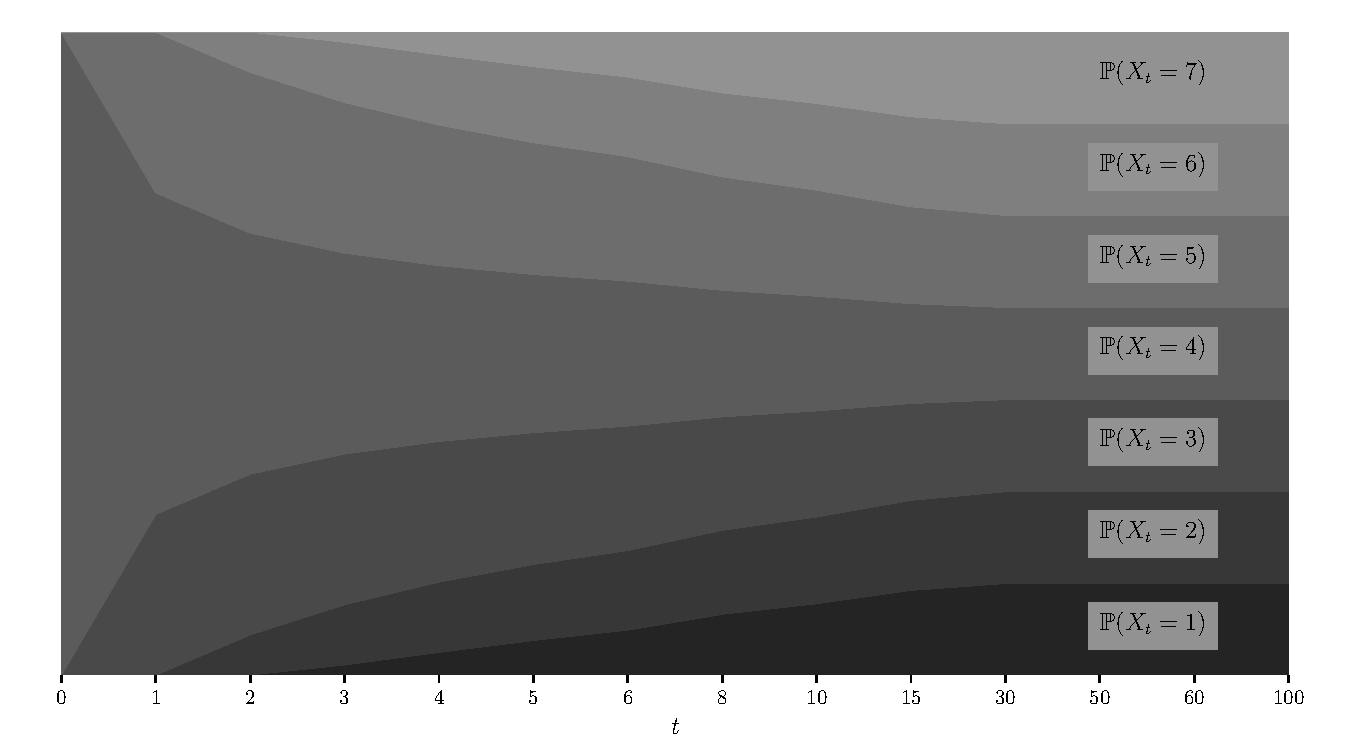
\includegraphics[height=8cm, center]{lrw.pdf}
                           	
		\subsubsection{Transience and Recurrence *}
			A final property of Markov chains we will examine is that of recurrence. It may be of
			interest how often a particular state is reached by a Markov chain, which leads to the
			question of whether a state will be entered infinitely often in the limit.
			\begin{definition}
				In a Markov chain with state space $\mathcal{I}$ and trantition matrix $\mathbf
				{P}$, state $i$ is \emph{recurrent} if $f_i \coloneqq \mathbb{P}(\tau^+_{i,i}
				< \infty) = 1$, and \emph{transient} if $f_i < 1$.
			\end{definition}
			\begin{comment}
				We call a Markov chain recurrent if all its states are recurrent themselves.
			\end{comment}
			
			We will see that this definition is equivalent to defining based on the expected number
			of visits to state $i$, but first we introduce the following notion:
			\begin{theorem}[Strong Markov Property]
				Suppose $(X_{t})_{t \in \mathbb{N}_0}$ is a Markov chain with state space
				$\mathcal{I}$, transition matrix $\mathbf{P}$.\\
				Then if $\tau$ is a stopping time, and we have $\tau = T$ for $T < \infty$, with
				$X_T = i$, then the stochastic process $(X_{T+k})_{k\in \mathbb{N}_0}$ is 
				Markov chain over $\mathcal{I}$, with transition matrix $\mathbf{P}$, and 
				initial distribution $\mu_j = \delta_{i,j}$, which is independent of the random
				variables $X_{0} \hdots X_{T-1}$.
			\end{theorem}
			The proof of the strong Markov property is beyond the scope of these notes, but the 
			result is useful for some computations. We now turn our attention to the proposition we 
			made earlier:
			\begin{lemma}
				A state $i$ of a Markov chain $(X_t)_{t \in \mathbb{N}_0}$ with state space 
				$\mathcal{I}$ and transition matrix $\mathbf{P}$ is recurrent if, and only if,
				$\mathbb{E}(N_i) = \infty$, where we define 
				$$
					N_i \coloneqq \sum_{t \in \mathbb{N}_0} 1[X_n = i | X_0 = i]
				$$
				Furthermore, this is the case if, and only if 
				$$	
					\sum_{t \in \mathbb{N}_0} (\mathbf{P}^{t})_{i,i} = \infty
				$$
			\end{lemma}
			\begin{proof}
				For some state $i \in  \mathcal{I}$, 
				by the strong Markov property, with $X_0 = i$, if $\tau^+_{i,i} = T < \infty$, 
				then the Markov chain `restarts' at $T$: Since $(X_{T+k})_{k \in \mathbb{N}_0}$ 
				has the same transition matrix, state space and initial distribution as the 
				original Markov chain, the first return time to $i$ in it will be finite with 
				the same probability as before, $f_i$, and since this event is independent of
				the past, we can deduce that the number of visits to $i$ follows a 
				\emph{geometric distribution} with parameter $f_i$, that is,
				$$
					\forall n \in \mathbb{N} . \mathbb{P}(N_i = n) = f_i^n \cdot (1-f_i)
				$$
				where we take the starting state $X_0 = i$ to be the first visit to $i$. The
				expected value of this is known to be $(1-f_i)^{-1}$, so recalling the 
				definition of recurrence, $i$ is thus recurrent iff $\mathbb{E}(N_i)=\infty$.
				\newline
				The second part of the lemma follows by taking expected values in the definition
				of $N_i$.
			\end{proof}

			We now examine whether whole Markov chains are recurrent. The first result we obtain is
			\begin{lemma}
				\label{lemma:commclrec}
				For any communicating class of states $C$, if any state $i$ in $C$ is recurrent,
				then all states in $C$ are.
			\end{lemma}
			\begin{proof}
				For a communicating class $C$, fix $i \neq j$ and suppose that $i$ is recurrent. 
				Note that since $i, j$ 
				communicate, $\exists n . p \coloneqq (\mathbf{P}^n)_{i,j} > 0$. Then, define 
				$$
					M_{i,j} \coloneqq \sum_{t \in \mathbb{N}_0} 1[X_t = i \land X_{t+n} = j]
				$$
				Note that $M_{i,j} \leq N_{i,j}$. Now, taking expected values, 
				\begin{align*}
					\mathbb{E}_i(M_{i,j}) &= \sum_{t \in \mathbb{N}_0} 
					\mathbb{P}(X_t = i \land X_{t+n} = j | X_0 = i) \\
					&= \sum_{t \in \mathbb{N}_0} \mathbb{P}(X_t = i | X_0 = i) \cdot 
					\mathbb{P}(X_{t+n} = j | X_t = i \land X_0 = i) \\
				\intertext{which is, by the strong Markov property,}
					&= p \cdot \sum_{t \in \mathbb{N}_0} \mathbb{P}(X_t = i | X_0=i)
				\end{align*}
				which is infinite since $p > 0$ and $i$ is recurrent. So if the Markov chain 
				ever enters state $i$ after starting in $X_0 = j$\footnote{note that we used
				the strong Markov property to make the notation simpler in the above 
				derivation}, the Markov chain returns to $j$ infinitely often, for any $j$ in
				$C$. Note that $C$ must be closed, since if it was open, there would be a 
				non-zero probability that, having started in $i$, the Markov would never reach 
				$i$ again since it left $C$ without ever being able to return. 
				This would imply $f_i < 1$, which contradicts our assumption. Therefore,
				by the Finite Hitting Theorem (and Markov's inequality), starting in $j$ the
				Markov chain will enter state $i$ in a finite number of steps with high 
				probability.
			\end{proof}

			From this result, we can draw an important conclusion without much difficulty:
			\begin{lemma}
				An irreducible Markov chain is either recurrent or transient (that is, if one
				state is recurrent, they all are, else they are all transient).\\
				Furthermore, a finite, irreducible Markov chain is always recurrent.
			\end{lemma}
			\begin{proof}
				The first part of the lemma follows straightforwardly from lemma 
				\ref{lemma:commclrec}, since the state space of an irreducible Markov chain is
				by definition a single communicating class. The second part, then, follows 
				simply since, if all states were transient, that is, $\exists N \in \mathbb{N}.
				\forall i\in\mathcal{I}, n \in \mathbb{N}. n > N \implies X_n \neq i$, then 
				$X_{N+1}$ could not take any values, which is impossible. Therefore, the states
				are not all transient, and are therefore all recurrent.
			\end{proof}

	\subsection{The Gambler's Ruin}
		We conclude this first look at Markov chains with a famous example: That of the `Gambler's 
		Ruin'. The Gambler's Ruin is a Markov chain on state space $\mathcal{I} \coloneqq\{0 \hdots 
		n\}$, where for a fixed probability
		$a$ the transtition matrix $\mathbf{P}$ has $P_{i, i+1} = a, P_{i, i-1} = b \coloneqq 1-a$, 
		where $0$ and $n$ are absorbing states. The usual interpretation is that a gambler repeatedly 
		bets a pound until they go bankrupt or reach a certain fortune, where the value $X_t$ typically
		represents the gambler's fortune at time $t$. \par

		\begin{lemma}
			Assuming the gambler starts with $s \in \mathcal{I}$ pounds, then let $\mathcal{E}$ 
			denote the even that the gambler reaches his goal of $n$ pounds before going bankrupt.
			Then
			$$
				\mathbb{P}(\mathcal{E}) = 
				\begin{dcases}
					\frac{1-(\sfrac{a}{b})^s}{1-(\sfrac{a}{b})^n} & a \neq b \\
					\frac{s}{n} & a = b = \sfrac{1}{2} 
				\end{dcases}
			$$
		\end{lemma}
		\begin{proof}
			Let $\tau \coloneqq \mathrm{inf}(t : X_t \in \{0, n\})$. Then it should be clear that
			$\mathcal{E} \equiv \langle X_\tau = n \angle$. Let also $p_i$ denote 
			$\mathbb{P}(X_\tau = n | X_0 = i)$. Then we have, by the (strong) Markov property, and 
			the law of total probability, that $p_i = ap_{i+1} + bp_{i-1}$. \\
			By recalling that $a+b = 1$ we can obtain $(\diamond)$
			\begin{align*}
				\forall i \in \{1 \hdots n-1\}. \\
				p_{i+1} - p_i &= \sfrac{b}{a} (p_i - p_i-1) \\
				              &= \hdots \\
				              &= (\sfrac{b}{a})^i p_1 \\
			\end{align*}
			Now, since obviously $p_{i+1} = p_{i+1} + p_{1} - p_1$, and expressing this as a 
			telescoping sum, we also arrive at $(\circ)$
			\begin{align*}
				p_{i+1} &= p_1 + \sum_{j=1}^{j=i} p_{j+1} - p_{j} \\
					&= p_1 + \sum_{j=1}^{j=i}(\sfrac{b}{a})^j p_1 & \text{by $(\diamond)$}\\
					&= p_1 \cdot 
					\begin{cases}
					p_1\cdot\frac{1-(\sfrac{b}{a})^{i+1}}{1-\sfrac{b}{a}} & a \neq b \\
						(i+1)p_1                                      & a = b
					\end{cases}
			\end{align*}
			Notice now that $p_n = 1$, then we obtain from $(\circ)$:
			\begin{align*}
				 1 &= p_n \\
				   &= 
			  	       \begin{cases}
			  	               \frac{1-(\sfrac{b}{a})^{n}}{1-\sfrac{b}{a}} & a \neq b \\
			  	               n\cdot p_1                                  & a = b
			  	       \end{cases}
				       \\
				\therefore \ \ \ \ \ \ \ \  
				p_1&= 	
			  	       \begin{cases}
			  	               \frac{1-\sfrac{b}{a}}{1-(\sfrac{b}{a})^{n}}   & a \neq b \\
			  	               \sfrac{1}{n}                                  & a = b
			  	       \end{cases}
			\end{align*}
			This, with $(\diamond)$, yields the result we set out to prove.
		\end{proof}


\section{Coupling and Convergence}
                           	
	\subsection{Total Variation Distance}
	Suppose we are throwing a coin, or rolling a die\footnote{The best thing about writing one's own 
	notes is that one may prevent the word `dice' being used to denote a singular form.}, of which we 
	do not know the probability measure over the sample space $\Omega$ (in the case of the coin, this
	might be $\Omega=\{\mathrm{Heads},\mathrm{Tails}\}$, and for the die, $\Omega=\{1,2,3,4,5,6\}$).
	At the moment, we have no means of expressing the `fairness' of such an experiment beyond the 
	dichotomy of the coin/die being `fair' (in case the distribution is uniform over all outcomes)
	or not (in case it is not). We would like to introduce some form of order modelling the 
	fairness of probability distributions relative to one another so as to be able to compare them 
	in more detail.

	To this end, we will define a \emph{metric} on the possible probability measures. The
	notion of metrics generalises the concept of distance for arbitrary sets. Formally,
	\begin{definition}[Metric Space]
		A \emph{metric space} is an ordered pair $\mathbf{M} \coloneqq (M, \Delta)$ of 
		a set $M$ and a total function $\Delta \in M^2 \rightarrow \mathbb{R}$ (known as
		a `metric'), abiding the axioms
		\begin{itemize}
			\item $\forall x,y \in M . \Delta(x,y) = 0 \iff x = y$
			\item $\forall x,y \in M . \Delta(x,y) = \Delta(y,x)$
			\item $\forall x,y,z \in M . \Delta(x,z) \leq \Delta(x,y)+\Delta(y,z)$
		\end{itemize}
	\end{definition}
	Note that from the definition it is easy to deduce that the metric $\Delta$ has a 
	non-negative range. 

	The specific metric we introduce for probability distributions over a \emph{enumerable} sample
	space $\Omega$ is the \emph{total variation distance}:
	\begin{definition}[Total Variation Distance]
		If $\Omega$ is a fixed, enumerable sample space, and $\mathfrak{P}$ is the set of 
		probability measures over $\Omega$, then we define the \emph{total variation distance}
		$d_{tv}$ to be the function
		$$
			d_{tv} \coloneqq \lambda (\mu, \eta) \in \mathfrak{P}^2 . \sfrac{1}{2} 
			\sum_{\omega \in \Omega} | \mu(\omega) - \eta(\omega) |
		$$
		and for any two such probability measures $\mu, \eta$ we denote $d_{tv}(\mu, \eta)$ as
		$\left\| \mu - \eta \right\|_{tv}$.
	\end{definition}
	From this definition it should be obvious that $(\mathfrak{P}, d_{tv})$ is a metric space for 
	any $\Omega$. We thus introduce a præorder $\preceq$ modelling the relative fairness of
	two probability measures defined by 
	$$
		\forall \mu, \eta \in \mathfrak{P}. 
		\mu \preceq \eta \stackrel{\mathrm{def}}{\iff} \|\mu - \upsilon\|_{tv} \geq 
		\|\eta - \upsilon\|_{tv}
	$$
	where we take $\upsilon$ to be the uniform distribution over $\Omega$, and if $\mu \preceq 
	\eta \land \eta \preceq \mu$, we say that $\mu, \eta$ are equally fair. For example, consider
	three six-sided dice, $H, M, N$, with probability distributions $\eta = \begin{pmatrix} 
	\sfrac{1}{3} & \sfrac{1}{12} & \sfrac{1}{12} &\sfrac{1}{12} &\sfrac{1}{12} & \sfrac{1}{3}
	\end{pmatrix}$, $\mu = \begin{pmatrix} \sfrac{1}{4} & \sfrac{1}{8} & \sfrac{1}{8} & 
	\sfrac{1}{8} & \sfrac{1}{8} & \sfrac{1}{4}\end{pmatrix}$ and $\nu = \begin{pmatrix} 
	\sfrac{1}{6} & \sfrac{1}{6} & \sfrac{1}{8} & \sfrac{1}{8} & \sfrac{1}{8} & \sfrac{9}{24}
	\end{pmatrix}$, respectively. Now we determine that
	\begin{itemize}
		\item $\|\eta - \upsilon\|_{tv} = \sfrac{1}{2} \left(2|\sfrac{1}{3} - \sfrac{1}{6}| + 
		4|\sfrac{1}{12}-\sfrac{1}{6}|\right) = \sfrac{1}{3}$
		\item $\|\mu - \upsilon\|_{tv} = \sfrac{1}{2} \left(2|\sfrac{1}{4} - \sfrac{1}{6}| + 
		4|\sfrac{1}{8}-\sfrac{1}{6}|\right) = \sfrac{1}{6}$
		\item $\|\nu - \upsilon\|_{tv} = \sfrac{1}{2} \left(|\sfrac{9}{24} - \sfrac{1}{6}| + 
		3|\sfrac{1}{8}-\sfrac{1}{6}|\right) = \sfrac{1}{6}$
	\end{itemize}
	So $\eta \preceq \mu \genfrac{}{}{0pt}{}{\preceq}{\succeq} \nu$, that is, $H$ is the `least 
	fair' of these dice, whilst $M$ and $N$ are equally fair.

	Note that there is an alternative way of computing the total variation distance between
	probability measures $\mu, \eta$\footnote{Remember from the definition of a probability space
	that a probability measure is a function from \emph{subsets}, not just members, of the sample
	space.}, given by lemma \ref{lemma:tvsup}.
	\begin{lemma}
		\label{lemma:tvsup}
		If $\Omega$ is an enumerable sample space, and $\mu, \eta$ are probability measures
		on $\Omega$, then 
		$$
			\|\mu - \eta\|_{tv} = \max_{\Theta \subseteq \Omega}|\mu(\Theta)-
			\eta(\Theta)|
		$$
	\end{lemma}
	\begin{proof}
		We prove the lemma by determining the value of $\max_{\Theta \subseteq \Omega}|\mu
		(\Theta) - \eta(\Theta)|$. To this end, we draw the reader's attention to the fact 
		that (two of) the subsets of $\Omega$ that maximise the given expression are $\Omega^+ 
		\coloneqq \{\omega \in \Omega : \mu(\omega) > \eta(\omega)\}$ and $\Omega^-\coloneqq
		\{\omega \in \Omega : \eta(\omega) > \mu(\omega)\}$. We prove this assertion first.
		\\
		Suppose that $\Theta$ maximises $|\mu(\Theta) - \eta(\Theta)|$, then note that either
		if for some $\omega_1, \omega_2 \in \Theta$, $\omega_1\in\Omega^+\land\omega_2\in
		\Omega^-$, we could increase the value of the given expression by removing one of the
		two outcomes, since 
		\begin{align*}
			&|\mu(\Theta) - \eta(\Theta)| \\
			=&|\mu(\Theta\setminus\{\omega_{2}\})-\eta(\Theta\setminus\{\omega_{2}\})
			+\mu(\omega_2)-\eta(\omega_2) | \\
			<&|\mu(\Theta\setminus\{\omega_2\})-\eta(\Theta\setminus\{\omega_2\})|\\
		\end{align*}
		(where a similar argument resting on $|x| = |-x|$ would increase the expression if 
		we removed $\omega_1$). Therefore, if $\Theta$ contains an element from $\Omega^+$,
		it does not contain any from $\Omega^-$, and vice versa. Now, since if it contained 
		no elements of either, the expression would have value $0$ and could be increased by 
		adding elements of either set, it must contain members of one of the two.
		\\
		Now note that if $\Omega^+ \not\subseteq \Theta$, 
		we can yet again increase the expression by adding those members of $\Omega^+$ not 
		already in $\Theta$, which again contradicts the assumption that $\Theta$ maximises
		the given expression. Due to a similar argument for $\Omega^-$, $\Theta$ contains 
		either all members of $\Omega^+$ or those of $\Omega^-$. Since adding to or removing 
		from $\Theta$ those outcomes in neither one of the sets does not change the value of 
		the expression, $\Theta$ might be $\Omega^+$ or $\Omega^-$. We prove that both of
		$\Omega^+$ and $\Omega^-$ maximise this expression by noticing that 
		$|\mu(\Omega^+) - \eta(\Omega^+)| = |\mu(\Omega^-) - \eta(\Omega^-)|$ since
		\begin{align*}
			\mu(\Omega^+)+\mu(\Omega^-)+\mu(\{\omega\in\Omega:\mu(\omega)=\eta(\omega)\})
			&= \eta(\Omega^+)+\eta(\Omega^-)+\eta(\{\omega\in\Omega:\mu(\omega)=
			\eta(\omega)\})\\
			\therefore\ \ \ 
			\mu(\Omega^+)+\mu(\Omega^-)&= \eta(\Omega^+)+\eta(\Omega^-)\\
			\therefore\ \ \ 
			\mu(\Omega^+) - \eta(\Omega^-)&= \eta(\Omega^-) - \mu(\Omega^+)
		\end{align*}
		Therefore, since the given expression takes the same value for both $\Omega^+,
		\Omega^-$, both of them maximise the expression, concluding the proof of the 
		assertion we made earlier. \par
		We can now easily conclude the proof of the lemma by:
		\begin{align*}
			\|\mu-\eta\|_{tv} &=\sfrac{1}{2}\sum_{\omega \in \Omega}|\mu(\omega)-
			\eta(\omega)|\\
			&= \sfrac{1}{2} \cdot \left(\sum_{\omega\in\Omega^+}(\mu(\omega) - 
			\eta(\omega)) + \sum_{\omega\in\Omega^-}(\eta(\omega) -\mu(\omega))\right)\\
			&= \sfrac{1}{2} \cdot 2 \cdot |\mu(\Omega^+) - \eta(\Omega^-)| \\
			&= \max_{\Theta \subseteq \Omega}(|\mu(\Theta)-\eta(\Theta)|)
		\end{align*}
	\end{proof}
	
	Take now $\mathbf{p}^t_\mu$ to be the probability distribution $X_t$ over the state space 
	$\mathcal{I}$ of a Markov chain given that $X_0 \sim \mu$, that is $\mathbf{p}^t_\mu = 
	\mu \cdot \mathbf{P}^t$. Then, if the Markov chain has stationary distribution $\pi$ we 
	have that $\|\mathbf{p}^t_\mu - \pi\|_{tv} \leq \max_{\nu}\|\mathbf{p}^t_r\nu 
	- \pi\|_{tv}$. We will use this to rephrase the Convergence Theorem from before, which will 
	allow us to prove it using a technique known as \emph{coupling}.

	\subsection{Coupling}
	Suppose we
	are observing two random variables $M, H$, with distibutions $\mu, \eta$, respectively, over
	the same probability space. Then we may wish to prove that $M$ and $H$ have certain properties 
	relative to each other, for example \emph{stochastic domination}:
	\begin{definition}[Stochastic Domination]
		If $X, Y$ are random variables, we say that $X$ dominates $Y$ stochastically, or that
		$Y$ is \emph{stochastically smaller}, iff $\forall x \in \mathbb{R}. \mathbb{P}(X>x)
		\geq \mathbb{P}(Y > x)$. We denote this as $Y \preccurlyeq X$. 
	\end{definition}

	For example, we may consider two weighted coins $C, K$ thrown a large number of times, 
	with probabilities of turning up heads at each throw of $\sfrac{1}{2}$ and $\sfrac{2}{3}$, 
	respectively. It is intuitive that $K$ should 
	thus stochastically dominate $C$, but this can be difficult to prove combinatorically. The
	technique known as \emph{coupling} circumvents this difficulty. 
	\begin{definition}
		Suppose $X,Y$ are random variables over sample spaces $\Omega, \Theta$, with 
		enumerable ranges. We call a random variable $Z = (X', Y')$ over the product space 
		$\Omega \times \Theta$\footnote{The probability space becomes modified by this, so 
		the variable $Z$ is measured by a different probability measure than $X,Y$. Call 
		this probability measure $\mathbb{P}'$.} a \emph{coupling} of $(X, Y)$ if the 
		marginal distribution of $X'$ is the distribution 
		of $X$, and the same holds for $Y'$ and $Y$---that is,
		$$
			\forall x \in \mathrm{range}(X).
			\sum_{y \in \mathrm{range}(Y)} \mathrm{Pr}_Z(x, y) = \mathrm{Pr}_X(x)
		$$
		and
		$$
			\forall y \in \mathrm{range}(Y).
			\sum_{x \in\\ \mathrm{range}(X)} \mathrm{Pr}_Z(x, y) = \mathrm{Pr}_Y(y)
		$$
	\end{definition}

	We can now state the following lemma:
	\begin{lemma}
		\label{lemma:stochdomcoup}
		Let $X$ and $Y$ be random variables over the same probability space. Then
		$Y \preccurlyeq X$ if, and only if, there is a coupling $(X', Y')$ of the two such
		that $\mathbb{P}'(Y' \leq X') = 1$.
	\end{lemma}
	\begin{comment}
		We will not prove this lemma in completeness; luckily the interesting direction
		for us is fairly easy to see: If such a coupling exists, then 
		\begin{align*}
			\mathbb{P}(x < Y) &= \mathbb{P}'(x < Y') \\
			&= \mathbb{P}'(x < Y'\land Y'\leq X') \\
			&\leq \mathbb{P}'(x < X') \\
			&= \mathbb{P}(x < X)
		\end{align*}
	\end{comment}

	To see why this is useful, consider now again our two weighted coins, and consider coupling 
	them as follows. Define $(X', Y') \coloneqq (X, X \lor Z)$, where $Z$ is a weighted coin 
	with probability $\sfrac{1}{3}$ of turning up heads. We can see that this is a coupling as 
	\begin{align*}
		\mathbb{P}'(Y' = \mathrm{Heads}) &= \mathbb{P}(X=\mathrm{Heads}) + 
		\mathbb{P'}(X = \mathrm{Tails}, Z = \mathrm{Heads}) \\
		&= \sfrac{1}{2} + \sfrac{1}{2} \cdot \sfrac{1}{3} = \sfrac{2}{3}
	\end{align*}
	Thus the marginal distribution of $Y'$ is the distribution of $Y$. That the same is true for
	$X'$ and $X$ is obvious, so we do indeeed have a coupling of the two variables. It is also
	obvious that $\mathbb{P}'(X' \leq Y')$, so we have proved that $X \preccurlyeq Y$ by lemma 
	\ref{lemma:stochdomcoup}.

	\subsubsection{The Coupling Lemma}

	Another useful property of couplings is that they provide a way of bounding the total 
	variation distance of two distributions; this result is known as the \emph{coupling lemma}.
	\begin{lemma}[Coupling Lemma]
		\label{lemma:coupling}
		Suppose $X$ and $Y$ are random variables with the same enumerable range in the same 
		probability space, and suppose
		that $\mu, \eta$ are probability distributions such that $X \sim \mu, Y \sim \eta$.
		Then if $(X',Y')$ is a coupling of $(X, Y)$, we have that 
		$$
			\|\mu, \eta\|_{tv} \leq \mathbb{P}'(X' \neq Y')
		$$
		Furhermore, it is always possible to find a coupling such that this is an 
		equivalence.
	\end{lemma}
	\begin{proof}
		Let the probability space containing $X, Y$ be $(\Omega, \mathcal{F}, \mathbb{P})$,
		and that containing $(X',Y')$ $(\Omega^2, \mathcal{F}', \mathbb{P}')$\footnote{Note 
		that the coupling is a single random variable over a sample space of ordered pairs, 
		returning 2-dimensional vectors of numbers,and that we implicitly define $X', Y'$ to 
		be the random variables returning the projection of the coupling onto the relevant 
		axes.} Now note that
		\begin{align*}
			\mu(x) &= \mathbb{P}(X=x) \\
			       &= \mathbb{P}'(X'=x) \\
			       &= \mathbb{P}'(X'=x \land Y'=X') + \mathbb{P}'(X'=x \land Y'\neq X')\\
			       &= \mathbb{P}'(Y'=x \land Y'=X') + \mathbb{P}'(X'=x \land Y'\neq X')\\
			       &\leq \eta(x) + \mathbb{P}'(X'=x, \land Y'\neq X')
		\end{align*}
		Similarly, we obtain $\eta(x) = \leq \mu(x) + \mathbb{P}'(Y'=x\land X'\neq Y')$.

		If we define $\rho \coloneqq \mathrm{range}(X)$, then we define the sets $\varrho^+ 
		\coloneqq \{x \in \rho : \mu(x) \geq \eta(x)\}$ and $\varrho^- \coloneqq
		\{x \in \rho : \mu(x) < \rho(x)\}$. Now, observe that by parts (2) and (4) of 
		lemma \ref{lemma:basicprobs}, we have that 
		\begin{align*}
			2 \cdot \|\mu - \eta\|_{tv} &= \sum_{x \in \rho} |\mu(x) - \eta(x)| \\
			&= \sum_{x \in \varrho^+} (\mu(x) - \eta(x)) + 
			   \sum_{x \in \varrho^-} (\eta(x) - \eta(x)) \\
			&\leq \sum_{x \in \varrho^+} \mathbb{P}'(X'=x \land Y' \neq X') 
			+ \sum_{x \in \varrho^-} \mathbb{P}'(Y'=x \land Y' \neq X') \\
			&\leq 2 \cdot \mathbb{P}'(X' \neq Y')
		\end{align*}

		So we have proven the first part of the lemma. We will prove the second part by 
		explicitly defining a coupling $(X', Y')$ of $(X,Y)$ such that the equality holds.
		To this end consider a coupling that follows the distribution $\nu$ as defined below:
		$$
			\nu(x,y) \coloneqq 
			\begin{dcases}
				\min(\mu(x), \eta(x)) & \text{if $x=y$}\\
				\frac{\max(\mu(x)-\eta(x),0)\cdot\max(\mu(y)-\eta(y), 0)}
				{\|\mu - \eta\|_{tv}} & \text{otherwise}
			\end{dcases}
		$$
		Where we will gloss over the fact that it is not obvious this is a valid coupling.
		However, note that
		\begin{align*}
			\mathbb{P}'(X' = Y') &= \sum_{x \in \rho} \nu(x,x) \\
			&= \sum_{x \in \rho} \min(\mu(x), \eta(x)) \\
			&= \sum_{x \in \varrho^+} \eta(x) + \sum_{x \in \varrho^-} \mu(x) \\
			&= \eta(\varrho^+) + \mu(\varrho^-) \\
			&= 1 - (\mu(\varrho^+)-\eta(\varrho^+)) \\
			&= 1 - \|\mu - \eta\|_{tv}
		\end{align*}
	\end{proof}

	\subsubsection{Coupling of Markov Chains}
	We can also couple Markov chains to prove that they have interesting properties. In the 
	case of Markov chains, we define coupling slightly differently:
	\begin{definition}
		If $(X_t)_{t \in \mathbb{N}_0}$ and $(Y_s)_{s \in \mathbb{N}_0}$ are Markov chains
		over state spaces $\mathcal{I}, \mathcal{J}$, respectively, then a coupling of 
		$((X_t)_{t\in \mathbb{N}_0},(Y_s)_{s\in \mathbb{N}_0})$ is a Markov chain 
		$(Z_t)_{t \in \mathbb{N}_0} \coloneqq (X'_t, Y'_t)_{t \in \mathbb{N}_0}$ over state 
		space $\mathcal{I}\times\mathcal{J}$, such that
		\begin{align*}
			\mathbb{P}'(X'_{t+1} = x' | Z_t = (x,y))&=\mathbb{P}(X_{t+1}=x'|X_t=x) \\
			\mathbb{P}'(Y'_{t+1} = y' | Z_t = (x,y))&=\mathbb{P}(Y_{t+1}=y'|Y_t=y) 
		\end{align*}
	\end{definition}

	One interesting result we can use the coupling of Markov chains for is to show that, in 
	a random walk over the integer plane, if two such random walks occur simultan\"eously, 
	starting at fixed, distinct locations, as time tends to the limit (that is, $t\rightarrow
	\infty$), it is immaterial what the starting locations were: If we construct a coupling such 
	that one of the two random walks proceeds as normal, while the other mimics its vertical 
	movement and mirrors its horizontal movement until they have states $(x, y_1)$ and $(x,y_2)$,
	after which the second starts mimicking its horizontal movement but mirroring its vertical 
	movement until the two random walks meet, after which they are coupled to move together,
	then both walks will have been `under the impression' of being truly random at all times, 
	but they end up walking together with high probability, regardless of their starting 
	positions. \par \ 

	We will consider a different example in detail: Consider a house inhabited by a family who
	own a cat (which, loath though one should be to give such foul creatures names, we will call 
	`Tom'). The house, and the family, is haunted by an invidious pestilence that makes cats
	seem almost agree\"able, which Tom is trying to rid his loving family of (we shall refer 
	to this creature as `Jerry'). We shall model this house as $C_3$, as though it comprised
	a garden, a living room and a garage, each of which is accessible to both Tom and Jerry
	from the other two, and we shall model each of their behaviours as simple random walks 
	through the house. Now, it may be of interest whether it is conceivably possible that Jerry
	evades Tom in perpetuity. This rather unenviable outcome is the result of coupling the two
	random walks as follows. Tom proceeds normally, while Jerry always mimics Tom's movements 
	relative to his earlier position. With these rules, since Tom is valiant enough never to 
	rest in one part of the house for more than one time step, Jerry will evade Tom until he
	dies of exhaustion rather than being braught to justice by Tom (Tom can, due to his larger
	physical size, and more certain food supply, be assumed to outlast Jerry in a war of 
	attrition). It remains to show that this is a valid coupling.

	\noindent In fact, we have that, obviously the marginal distribution of $T'_{t+1}$ as 
	conditioned on $(T'_t, J'_t)$ is correct. It follows that if $x,y$ are distinct parts of
	the house (and $z$ might be), then $\mathbb{P}'(J'_{t+1} = x | (T'_t, J'_t) = (z,y)) = 
	\mathbb{P}'(T'_{t-1} - T'_t \equiv x-y \pmod 3) = \sfrac{1}{2}$, so even Jerry's marginal
	distribution is correct. Below, we have given the Markov chain as a node-and-link diagram
	to make this admittedly contrived, informal, and altogether meaningless example slightly 
	more clear\footnote{As a way to justify the author's hatred (which may or may not have been
	evident) for this example, note that the lecture slides are so bad in this place that they
	give wrong transition probabilities for the states the coupling is not meant to enter, 
	when there are actually trivial right ones available.}.
	%TODO----Finish up this heaping pile of shit
	\begin{center}
	\begin{tikzpicture}[node distance=2.25cm]
		\draw node[circle,minimum size=1.0cm, draw] (10) {$(1,0)$};
		\draw node[above right of=10] (h) {};
		\draw node[circle,minimum size=1.0cm, draw, right of=h, node distance=1cm](21)
		{$(2,1)$};
		\draw node[circle,minimum size=1.0cm, draw, above left of=h] (02) {$(0,2)$};
		\draw[->] (02) edge [bend right] node[pos=0.5, left] {$\sfrac{1}{2}$} (10);
		\draw[->] (10) edge node[pos=0.5, right] {$\sfrac{1}{2}$} (02);
		\draw[->] (21) edge [bend right] node[pos=0.5, above] {$\sfrac{1}{2}$} (02);
		\draw[->] (02) edge  node[pos=0.5, below] {$\sfrac{1}{2}$} (21);
		\draw[->] (21) edge node[pos=0.5, above] {$\sfrac{1}{2}$} (10);
		\draw[->] (10) edge [bend right] node[pos=0.5, below] {$\sfrac{1}{2}$} (21);
		\draw node[circle, minimum size=1.0cm, draw, right of=21] (11) {$(1,1)$};
		\draw node[circle, minimum size=1.0cm, draw, above of=11] (00) {$(0,0)$};
		\draw node[circle, minimum size=1.0cm, draw, below of=11] (22) {$(2,2)$};
		\draw[->] (22) edge [bend right] node[pos=0.5,right] {$\sfrac{1}{2}$} (11);
		\draw[->] (11) edge [bend right] node[pos=0.5, left] {$\sfrac{1}{2}$} (22);
		\draw[->] (22) edge [out=35, in=325] node[pos=0.5, left] {$\sfrac{1}{2}$} (00);
		\draw[->] (00) edge [out=215, in=145] node[pos=0.5, right] {$\sfrac{1}{2}$} (22);
		\draw[->] (11) edge [bend right] node[pos=0.5, right] {$\sfrac{1}{2}$} (00);
		\draw[->] (00) edge [bend right] node[pos=0.5, left] {$\sfrac{1}{2}$} (11);
		\draw node[circle,minimum size=1.0cm, draw, right of=11](12)
		{$(1,2)$};
		\draw node[right of=12, node distance=1cm] (h2) {};
		\draw node[circle,minimum size=1.0cm, draw, below right of=h2] (01) {$(0,1)$};
		\draw node[circle,minimum size=1.0cm, draw, above right of=h2] (20) {$(2,0)$};
		\draw[->] (20) edge [bend left] node[pos=0.5, right] {$\sfrac{1}{2}$} (01);
		\draw[->] (01) edge node[pos=0.5, left] {$\sfrac{1}{2}$} (20);
		\draw[->] (12) edge [bend left] node[pos=0.5, above] {$\sfrac{1}{2}$} (20);
		\draw[->] (20) edge  node[pos=0.5, below] {$\sfrac{1}{2}$} (12);
		\draw[->] (12) edge node[pos=0.5, above] {$\sfrac{1}{2}$} (01);
		\draw[->] (01) edge [bend left] node[pos=0.5, below] {$\sfrac{1}{2}$} (12);
	\end{tikzpicture}
	\end{center}

	\subsection{Convergence Theorem (Reprise)}
	As previously mentioned, we have that, for any intial distribution $\mu$, $\|
	\mathbf{p}_\mu^t-\pi \|_{tv} \leq \max_\nu \|\mathbf{p}_\nu^t-\pi\|_{tv}$. Recall the 
	Convergence Theorem from before:
	\begin{reptheorem}{theorem:convergence}[COnvergence Theorem]
		If $(X_t)_{t \in \mathbb{N}_0}$ is an aperiodic, irreducible Markov chain over
		finite state space $\mathcal{I}$, then if its stationary distribution is $\pi$,
		$$
			\forall i, j \in \mathcal{I} . \lim_{t \rightarrow \infty} 
			(\mathbf{P}^t)_{i,j} = \pi_j
		$$
	\end{reptheorem}
	Now, recall that the total variation distance is a metric on the set of probability 
	distributions over $\mathcal{I}$, so $\|\mu - \eta\|_{tv} = 0 \iff \mu = \eta$.
	This means that, with the limit from before, we can rephrase the above theorem as follows:
	\begin{reptheorem}{theorem:convergence}
		If $(X_t)_{t \in \mathbb{N}_0}$ is an aperiodic, irreducible Markov chain over  
		finite state space $\mathcal{I}$, then if its stationary distribution is $\pi$,
		$$
			\lim_{t\rightarrow\infty} \max_{\nu} \|\mathbf{p}_\nu^t - \pi\|_{tv} = 0
		$$
	\end{reptheorem}

	\emph{Finally}, using coupling, we will prove that this is indeed a theorem.
	\begin{proof}
		Take $(Y_t)_{t \in \mathbb{N}_0}$ to be a Markov chain over the same state space
		$\mathcal{I}$, with the same transition matrix $\mathbf{P}$ as $(X_t)_{t\in
		\mathbb{N}_0}$ (informally, think of this new Markov chain as a copy of the first
		one). However, let $X_0 \sim \mu$, for some probability distribution $\mu$ over 
		$\mathcal{I}$, and let $Y_0 \sim \pi$.\par
		We now introduce the so-called \emph{Doblin Coupling}, a coupling 
		$(X'_t, Y'_t)_{t\in\mathbb{N}_0}$ of the Markov 
		chains $((X_t)_{t\in\mathbb{N}_0}, (Y_s)_{s \in \mathbb{N}_0})$ the transition
		matrix of which is given by 
		$$
			P'_{(x_1, y_1), (x_2, y_2)} = 
			\begin{dcases}
				P_{x_1, x_2} \cdot P_{y_1, y_2} & \text{if $x_1\neq y_1$} \\
				P_{x_1, x_2} & \text{if $(x_1, x_2) = (y_1, y_2)$} \\
				0 & \text{otherwise}
			\end{dcases}
		$$
		It should be reasonable simple to verify that this is a valid coupling for the two 
		Markov chains. Now, notice that since the original Markov chains were both 
		aperiodic, finite and irreducible, $\exists T \in \mathbb{N}. \forall i, j \in 
		\mathcal{I}. (\mathbf{P}^T)_{i,j} > 0$. Now while the reader may wonder if, and why 
		this is actually true, we draw their attention to the fact that we are waving our 
		hands profucsely and no-one need worry\footnote{This claim is actually true; it
		is proven in the problems' class. However, the proof relies entirely on a fact
		that is ridiculous to assume as knowledge, and that is \emph{not} proven there
		(although it is not very difficult to prove).}.
		\\
		So take $\epsilon\coloneqq \min_{i,j \in \mathcal{I}} (\mathbf{P}^T)_{i,j}$, and 
		note that therefore $(\mathbf{P}^T)_{i,j} \cdot(\mathbf{P}^T)_{k,j} \geq \epsilon^2 
		> 0$ for all $i,j,k \in \mathcal{I}$. Thus, the coupling will have $\mathbb{P}(X'_T 
		= Y_T') \geq \epsilon^2$, so by the strong Markov property, $\forall k \in 
		\mathbb{N}. \mathbb{P}(X'_{kT} \neq Y'_{kT}) \leq (1-\epsilon^2)^k$. So, by the 
		Coupling Lemma, for any intial distribution $\mu$, since $\forall t . \mathbf{p}
		_\pi^t = \pi$,
		$$
			\|\mathbf{p}^t_{\mu} - \pi\|_{tv} \leq \mathbb{P}(X'_t \neq Y'_t)
		$$
		which tends to 0 as $t \rightarrow \infty$.
	\end{proof}
	\begin{comment}
		Note that, with the Convergence Theorem, we have a way of determining $\mathbf{P}
		^\infty$---$\forall i, j \in \mathcal{I}. (\mathbf{P}^\infty)_{i,j} = \pi_j$.
		This is because it holds for all initial distributions, so in particular it holds
		for those where $\mu(i) = 1$ for some state $i$. The result follows from there.
	\end{comment}

	\subsubsection{Applications of the Convergence Theorem}
		The convergence theorem is a powerful property of such Markov chains. It allows us 
		to approximate sampling from certain distributions by constructing a randomised 
		process that behaves as a Markov chain with the desired stationary distribution.
		For example, suppose we have a bipartite graph $G$, and we wish to sample a 
		matching uniformly. We can use the following algorithm:
		\begin{lstlisting}[caption=Matching Generator,language=python,style=mystyle]
M = pick(some matching)          # e.g. empty
for _ in range(x):               # some largeish number of iterations
	if(random > 0.5):
		continue
	else:
		u,v = random.choice(E)
		if u,v in M:
			M.remove(u,v)
		elif M.extensible(u,v):
			M.add(u,v)
		elif any((u', v') in M, u'=u or v'=v):
			M.remove(u',v')
			M.add(u,v)
		else:
			continue
		\end{lstlisting}
		This example, rather informally, works as a Markov chain on the matchings in $G$, 
		where from any one matching, the transition probabilities are uniformly 
		distributed among those matchings obtainable from adding one edge, removing an 
		edge, replacing one (or perhaps two) edges, or not modifying the matching at all
		\footnote{weighted by $\sfrac{1}{2}$ to make the Markov chain aperiodic. With a 
		finite $G$, this will lead to the necessary properties.}. This leads to a Markov
		chain with a uniform stationary distribution, so by running it for `long 
		enough', we will eventually have a matching that has been chosen uniformly at 
		random from all possible matchings of $G$. \par
		This is a helpful tool, but we currently do not hold an idea of how long 
		\emph{is} long enough. To answer that question, we consider the notion of mixing 
		times.

	\subsection{Mixing Time}
		The concept of a mixing time formalises the number of steps a Markov chain has 
		to make before being `closer' (with respect to total variation distance) than 
		some threshold to the stationary distribution. To be precise, we define
		\begin{definition}[Mixing Time]
			The \emph{Mixing Time} $\tau$ of a Markov chain with transition matrix 
			$\mathbf{P}$ and stationary distribution $\pi$ is defined as 
			$$
				\tau \coloneqq \lambda \epsilon \in \mathbb{R}^+ .
				\min(t \in \mathbb{N}_0 : d(t) \leq \epsilon)
			$$
			where we take $d \coloneqq \lambda t . \max_{i \in \mathcal{I}}
			\|\mathbf{p}^t_i - \pi\|_{tv}$. 
			We also define the notation $\overline{d} \coloneqq 
			\lambda t. \max_{i,j \in \mathcal{I}} \|\mathbf{p}^t_i - 
			\mathbf{p}^t_j\|_{tv}$.
		\end{definition}

		We say that $\tau(\epsilon)$ measures how long it takes before the Markov chain 
		is `$\epsilon$-close' to stationarity. Often, we take $\epsilon = \sfrac{1}{4}$,
		so often, in fact, that we further denote $t_\mathrm{mix} \coloneqq \tau(
		\sfrac{1}{4})$. We will prove some helpful properties of the mixing time now,
		specifically:
		\begin{claim}
			\begin{align*}
				\forall 0 < \epsilon < \delta < \sfrac{1}{2} . \\
				\tau(\epsilon) &\leq \left\lceil 
				\frac{\ln(\epsilon)}{\ln(2\delta)} \right\rceil \tau(\delta)\\
				\intertext{and}
				\forall \epsilon < \frac{1}{4} . \\
				\tau(\epsilon) &\leq \left\lceil \log_2 \epsilon^{-1}\right\rceil
				t_\mathrm{mix}
			\end{align*}
		\end{claim}
		Before we proceed with the proof, we would like to draw the reader's attention
		to the fact that these properties are merely stated in the lectures, \emph{not} 
		proven there. However, these are anything but obvious, and stating them without
		proof is not in the spirit in which these notes should be read.
		\\
		Before we may prove these claims, we must first prove two properties of the 
		functions $d, \overline d$ as defined earlier:
		\begin{lemma}
			For any $t \in \mathbb{N}_0$, and any Markov chain where the functions 
			$d, \overline d$ are well-defined,
			$$
				d(t) \leq \overline d(t) \leq 2 \cdot d(t)
			$$
		\end{lemma}
		\begin{proof}
			Note that, since the total variation distance is a metric on the space
			of probability distributions over the  state space of the Markov chain,
			by the triangle inequality (the third axiom we gave for a metric), and 
			the symmetry of the total variation distance that $\overline d(t) \leq 
			2 d(t)$. \\
			To show that $d(t) \leq \overline d(t)$, we require a certain amount
			more ingenu\"ity. We note that since $\pi$ is a stationary distribution
			for the Markov chain (which exists since $d$ is well-defined by our 
			hypothesis), we have that $\forall I \subset \mathcal{I}. \pi(I) = 
			\sum_{i \in I} \pi(i) \mathbf{p}_i^t(I)$. From there, we get
			\begin{align*}
				\intertext{By lemma \ref{lemma:tvsup},}
				d(t) \equiv
				\|\mathbf{p}^t_j - \pi\|_{tv} &= \max_{I \subseteq \mathcal{I}}
				| \mathbf{p}^t_j(I) - \pi(I)| \\
				&= \max_{I \subseteq \mathcal{I}}\left|\sum_{i \in \mathcal{I}}
				\pi(i)(\mathbf{p}^t_j(I) - \mathbf{p}^t_i(I))\right| \\
				&\leq \sum_{i \in \mathcal{I}} \pi(i) \max_{I \subseteq 
				\mathcal{I}} 
				\left|\mathbf{p}^t_j(I) - \mathbf{p}^t_i(I))\right| \\
				&= \sum_{i \in \mathcal{I}} \pi(i) \|\mathbf{p}^t_j - 
				\mathbf{p}^t_i\|_{tv} \\
				&\leq \max_{i,j \in \mathcal{I}}
				\|\mathbf{p}^t_i - \mathbf{p}^t_j\|_{tv}\\
				&\equiv \overline d(t)
			\end{align*}
		\end{proof}
		Secondly, we will need that $\overline d$ is \emph{submultiplicative}, that is,
		\begin{lemma}
			\label{lemma:dsubmul}
			For any $s,t \in \mathbb{N}_0$, $\overline d(s + t) \leq \overline d(s)
			\cdot \overline d(t)$.
		\end{lemma}
		\begin{proof}
			Let $(X_s, Y_s)_{s\in\mathbb{N}_0}$ be the coupling of our Markov chain
			with itself that achieves equality in the Coupling Lemma. That is,
			for fixed $i,j \in \mathcal{I}$, where we take $X_0 = i, Y_0 = j$,
			$$
				\|\mathbf{p}^s_i - \mathbf{p}_j^t \|_{tv} = \mathbb{P'}_{i,j}
				(X_s \neq Y_s)i
			$$
			Since $\mathbf{P}^{s+t} = \mathbf{P}^s \cdot \mathbf{P}^t$, we have
			that 
			$$	
				\forall{k \in \mathcal{I}}. (\mathbf{P}^{s+t})_{i,k}
				=\sum_{l \in \mathcal{I}} \mathbf{p}^s_i(l) (\mathbf{P}^t)_{l,k}
				=\mathbb{E}_i((\mathbf{P}^t)_{X_s, k})
			$$
			Similarly, we obtain $(\mathbf{P}^{s+t})_{j,k} = \mathbb{E}_j(
			(\mathbf{P}^t)_{Y_s, k})$.\\
			Therefore, we obtain
			\begin{align*}
				(\mathbf{P}^t)_{i,k} - (\mathbf{P}^t)_{j,k} &=
			\mathbb{E}_{i,j}((\mathbf{P}^t)_{X_s, k}-(\mathbf{P}^t)_{Y_s, k})\\
			\intertext{which we can use to arrive at}
			\|\mathbf{p}_i^{s+t} - \mathbf{p}_j^{s+t}\|_{tv} &= 
			\sfrac{1}{2} \sum_{k} |\mathbb{E}_{i,j}((\mathbf{P}^t)_{X_s, k}-
			(\mathbf{P}^t)_{Y_s, k})|\\
			&\leq \mathbb{E}_{i,j}\left(\sfrac{1}{2}\sum_{k}|(\mathbf{P}^t)_{X_s, 
			k}- (\mathbf{P}^t)_{Y_s, k})|\right) \\
			&= \mathbb{E}_{i,j}(\|\mathbf{p}^t_{X_s}-\mathbf{p}^t_{Y_s}\|_{tv})\\
			\intertext{which, since the distance is $0$ when $X_s=Y_s$,}
			&= \mathbb{E}_{i,j}(\|\mathbf{p}^t_{X_s}-\mathbf{p}^t_{Y_s}\|_{tv}
			\cdot 1[X_s \neq Y_s]) \\
			&\leq \overline d(t) \mathbb{E}_{i,j}(1[X_s \neq Y_s]) \\
			&= \overline d(t) \mathbb{P}_{i,j}(X_s \neq Y_s) \\
			\intertext{which, since the coupling is `optimal', is}
			&= \overline d(t) \|\mathbf{p}_i^s - \mathbf{p}_j^s\|_{tv}
			\end{align*}
			If we maximise both of these expressions over $i,j$ we obtain the 
			desired result.
		\end{proof}

		Now note that with lemma \ref{lemma:dsubmul}, we also clearly get that for any
		nonnegative integer $l$, we have that 
		$$
			d(l\cdot t) \leq \overline d(l\cdot t) \leq \overline{d}(t)^l.
		$$
		
		We can now proceed with the proof of the claims we made before.
		\begin{proof}
			Using the two lemmas we have just proven, we note that
			$$
				d(l\cdot\tau(\epsilon)) \leq \overline d(\tau(\epsilon))^l 
				\leq (2\cdot\epsilon)^l
			$$
			for any nonnegative integer $l$. Now,
			\begin{align*}
				\epsilon &< d(\tau(\epsilon) - 1) \\
				&\leq d\left(\left\lfloor\frac{\tau(\epsilon)-1}{\tau(\delta)}
				\right\rfloor\tau(\delta)\right)\\
				&\leq (2\delta)^{\left\lfloor\frac{\tau(\epsilon)-1}
				{\tau(\delta)}\right\rfloor} \\
			\intertext{Therefore,}
				\ln(\epsilon) &< \ln(2\delta) \cdot \left\lfloor\frac{\tau
				(\epsilon)-1}{\tau(\delta)}\right\rfloor \\
				\frac{\ln(\epsilon)}{\ln(2\delta)} &> \left\lfloor\frac{\tau
				(\epsilon)-1}{\tau(\delta)}\right\rfloor \\
				\left\lceil\frac{\ln(\epsilon)}{\ln(2\delta)} \right\rceil&> 
				\frac{\tau(\epsilon)-1}{\tau(\delta)} \\
				\left\lceil\frac{\ln(\epsilon)}{\ln(2\delta)} \right\rceil 
				\cdot \tau(\delta) &> \tau(\epsilon)-1 \\
			\intertext{So, since both sides are integer,}
				\left\lceil\frac{\ln(\epsilon)}{\ln(2\delta)} \right\rceil 
				\cdot \tau(\delta) &\geq \tau(\epsilon) 
			\end{align*}
			The second claim follows simply by setting $\delta=\sfrac{1}{4}$.
		\end{proof}

		We can further bound the mixing times of Markov chains using coupling, which
		is expressed in  the following lemma:
		\begin{lemma}[Coupling Lemma for Mixing]
			Let $(X_t)_{t\in\mathbb{N}_0}$ be a Markov chain on state space $\mathcal
			{I}$, with stationary distribution $\pi$. Then if $(Y_t,Z_t)_{t\in
			\mathbb{N}_0}$ is a coupling of this Markov
			chain ith itself, and there exists a $T\in\mathbb{N}$, and an $\epsilon>0$
			such that
			$$
				\forall i,j \in \mathcal{I}.
				\mathbb{P}_{x,y}(Y_T \neq Z_T) \leq \epsilon,
			$$
			then $\tau(\epsilon) \leq T$.
		\end{lemma}
		\begin{proof}
			Let $(Y_t, Z_t)_{t\in\mathbb{N}_0}$ be such a coupling, and suppose that
			$Y_0 = i, Z_0 \sim \pi$. For any $I \subseteq \mathcal{I}$, we have that
			\begin{align*}
				\mathbb{P}(Y_T \in I) &\geq \mathbb{P}(Z_T \in I \land Y_T=Z_T) \\
				&= 1 - \mathbb{P}(Z_T \neq Y_T \lor Z_T \notin I) \\
				&\geq 1 - \mathbb{P}(Z_T\notin I) - \mathbb{P}(Z_T \neq Y_T) \\
				&\geq \mathbb{P}(Z_T \in I) - \epsilon \\
				&= \pi(I) - \epsilon
			\end{align*}
			Now, from the same steps, we get that $\mathbb{P}(Y_T\notin\mathcal{I}
			\setminus I) \geq \pi(\mathcal{I}  \setminus I) - \epsilon$, from which we 
			may then obtain $\mathbb{P}(Y_T \in I) \geq \pi(I) + \epsilon$.\\
			This, in conjunction with the first bound, allows us to observe that
			$$
				d(T) = \max_{i\in \mathcal{I}}\max_{I\subseteq\mathcal{I}} 
				|\mathbf{p}^T_i(I)-\pi(I)| \leq \epsilon,
			$$ 
			so $\tau(\epsilon) \leq T$.
		\end{proof}
